\documentclass{beamer}
\usepackage[spanish,mexico]{babel}
\usepackage{graphicx,hyperref,ru,url}
\usepackage{textpos}
\usepackage{etoolbox}
\usepackage{amsfonts}
\usepackage{amsmath}
\usepackage{amstext}
\usepackage{amscd}
\usepackage{amsthm}
\usepackage{amsbsy}
\usepackage{amssymb}
\usepackage{appendix}
\usepackage{enumerate}
\usepackage{multirow}
\usepackage[mathscr]{eucal}
\usepackage{fancyhdr}
\usepackage{supertabular}
\usepackage{fancybox}
\usepackage{array}
\usepackage{booktabs}
\usepackage{soul}
\usepackage{epic}
\usepackage{float}
\usepackage{subcaption}
\usepackage{appendix}
% The title of the presentation:
%  - first a short version which is visible at the bottom of each slide;
%  - second the full title shown on the title slide;
\title[Numerical Solutions to the Stochastic and Deterministic Burgers' Equation by Spectral Methods.]{
  Numerical Solutions to the Stochastic and Deterministic Burgers' Equation by Spectral Methods.}

% Optional: a subtitle to be dispalyed on the title slide
%\subtitle{Show where you're from}

% The author(s) of the presentation:
%  - again first a short version to be displayed at the bottom;
%  - next the full list of authors, which may include contact information;
\author[Alan Daniel Matzumiya Zazueta]{
  Alan Daniel Matzumiya Zazueta \\\medskip
  {\small \url{alan.matzumiya@gmail.com}}}

% The institute:
%  - to start the name of the university as displayed on the top of each slide
%    this can be adjusted such that you can also create a Dutch version
%  - next the institute information as displayed on the title slide
\institute[Universidad de Sonora]{
  Universidad de Sonora}

% Add a date and possibly the name of the event to the slides
%  - again first a short version to be shown at the bottom of each slide
%  - second the full date and event name for the title slide
\date[\Today]{
  \Today}

\begin{document}

\begin{frame}
  \titlepage
\end{frame}

\begin{frame}	
	\begin{block}{Motivaci\'on}
	\begin{itemize}
		\only<1->{
			\item 
			Encontrar soluciones anal\'iticas de ecuaciones diferenciales muchas veces es complicado.  
		}
		\only<2->{
			\item 
			Son necesarias para estudiar sistemas complejos. 
		}
		\only<3->{
			\item 
			Los m\'etodos espectrales son una excelente alternativa para obtener aproximaciones de alta precisi\'on. 	
		}
		\only<4->{
			\item 
			Ademas, son faciles de implementar. 	
		}			
	\end{itemize}
\end{block}
\end{frame}

\begin{frame}
\begin{block}{Objetivos}
	\begin{itemize}	
		\only<1->{
		\item 
		Estudiar los fundamentos de los m\'etodos espectrales.
		}
		\only<2->{
		\item
		Implementarlos a la ecuaci\'on de Burgers' en su versi\'on determinista y estoc\'astica.
		}
		\only<3->{
		\item 
		Hacer estudios num\'ericos para evaluar el comportamiento, y la precisi\'on de estos m\'etodos.		
		}
	\end{itemize}
\end{block}
\end{frame}

\begin{frame}
  \frametitle{Contenido}

  \tableofcontents
\end{frame}

% Section titles are shown in at the top of the slides with the current section 
% highlighted. Note that the number of sections determines the size of the top 
% bar, and hence the university name and logo. If you do not add any sections 
% they will not be visible.
\section{Introducci\'on}
	\begin{frame}
\frametitle{Introducci\'on}
	\only<1->{
	La din\'amica de los fluidos incompresibles es descrita mediante las siguientes ecuaciones:
	}
	\only<2->{
	\begin{block}{Ecuaciones de Navier-Stokes}	
		\begin{equation*}
		\left \lbrace \begin{array}{ll}
		\nabla \cdot v = 0, \\
		(\rho v)_t + (\nabla \cdot \rho v) v + \nabla p - \mu \nabla^2 v - \rho G = 0.
		\end{array}  \right .
		\label{navierstokes}
		\end{equation*}
		$\rho =$ Densidad, $p =$ Presi\'on, $v =$ Velocidad, $\mu =$ Viscosidad.
	\end{block}
	En este caso, $G$ representa los efectos gravitacionales.
	}
\end{frame}

\begin{frame}
	\only<1->{
	Definiendo $x \in I \subset \mathbb{R}$, y $\alpha = \frac{\mu}{\rho}$; considerando $\rho, p, \mu =$ constantes.
	\begin{block}{Ecuacion de Burgers' (Formulaci\'on Fuerte)}
	\begin{equation*}
	\frac{\partial v(x, t)}{\partial t} +  \underbrace{v(x, t) \frac{\partial v(x, t)}{\partial x}}_{\textbf{Convecci\'on}} - \underbrace{\alpha \frac{\partial^2 v(x, t)}{\partial x^2}}_{\textbf{Difusi\'on}} - \hspace{1mm}g(x, t) = 0.
	\end{equation*}
	\end{block}
	}
	\only<2->{
	\begin{block}{Soluci\'on An\'alitica $(g \equiv 0)$}	
		\begin{equation*}
		v(x, t) =  \displaystyle \frac{\int_{-\infty}^{\infty} \frac{x - \xi}{t} \varphi_0 (\xi) e^{- \frac{(x - \xi)^2}{4 \alpha t}} d\xi}{\int_{-\infty}^{\infty} \varphi_0 (\xi) e^{- \frac{(x - \xi)^2}{4 \alpha t}} d\xi}, \hspace{2mm} \varphi_0 (\xi) = e^{- \int_{0}^{\xi} \frac{v_0 (y)}{2 \alpha} dy} 
		\end{equation*}
	\end{block}	
	}
\end{frame}

\begin{frame}
Condicion inicial $v_0 (x) = e^{-0.05x^2}$ y con $\alpha = 0.01$.
\begin{figure}
	\centering
	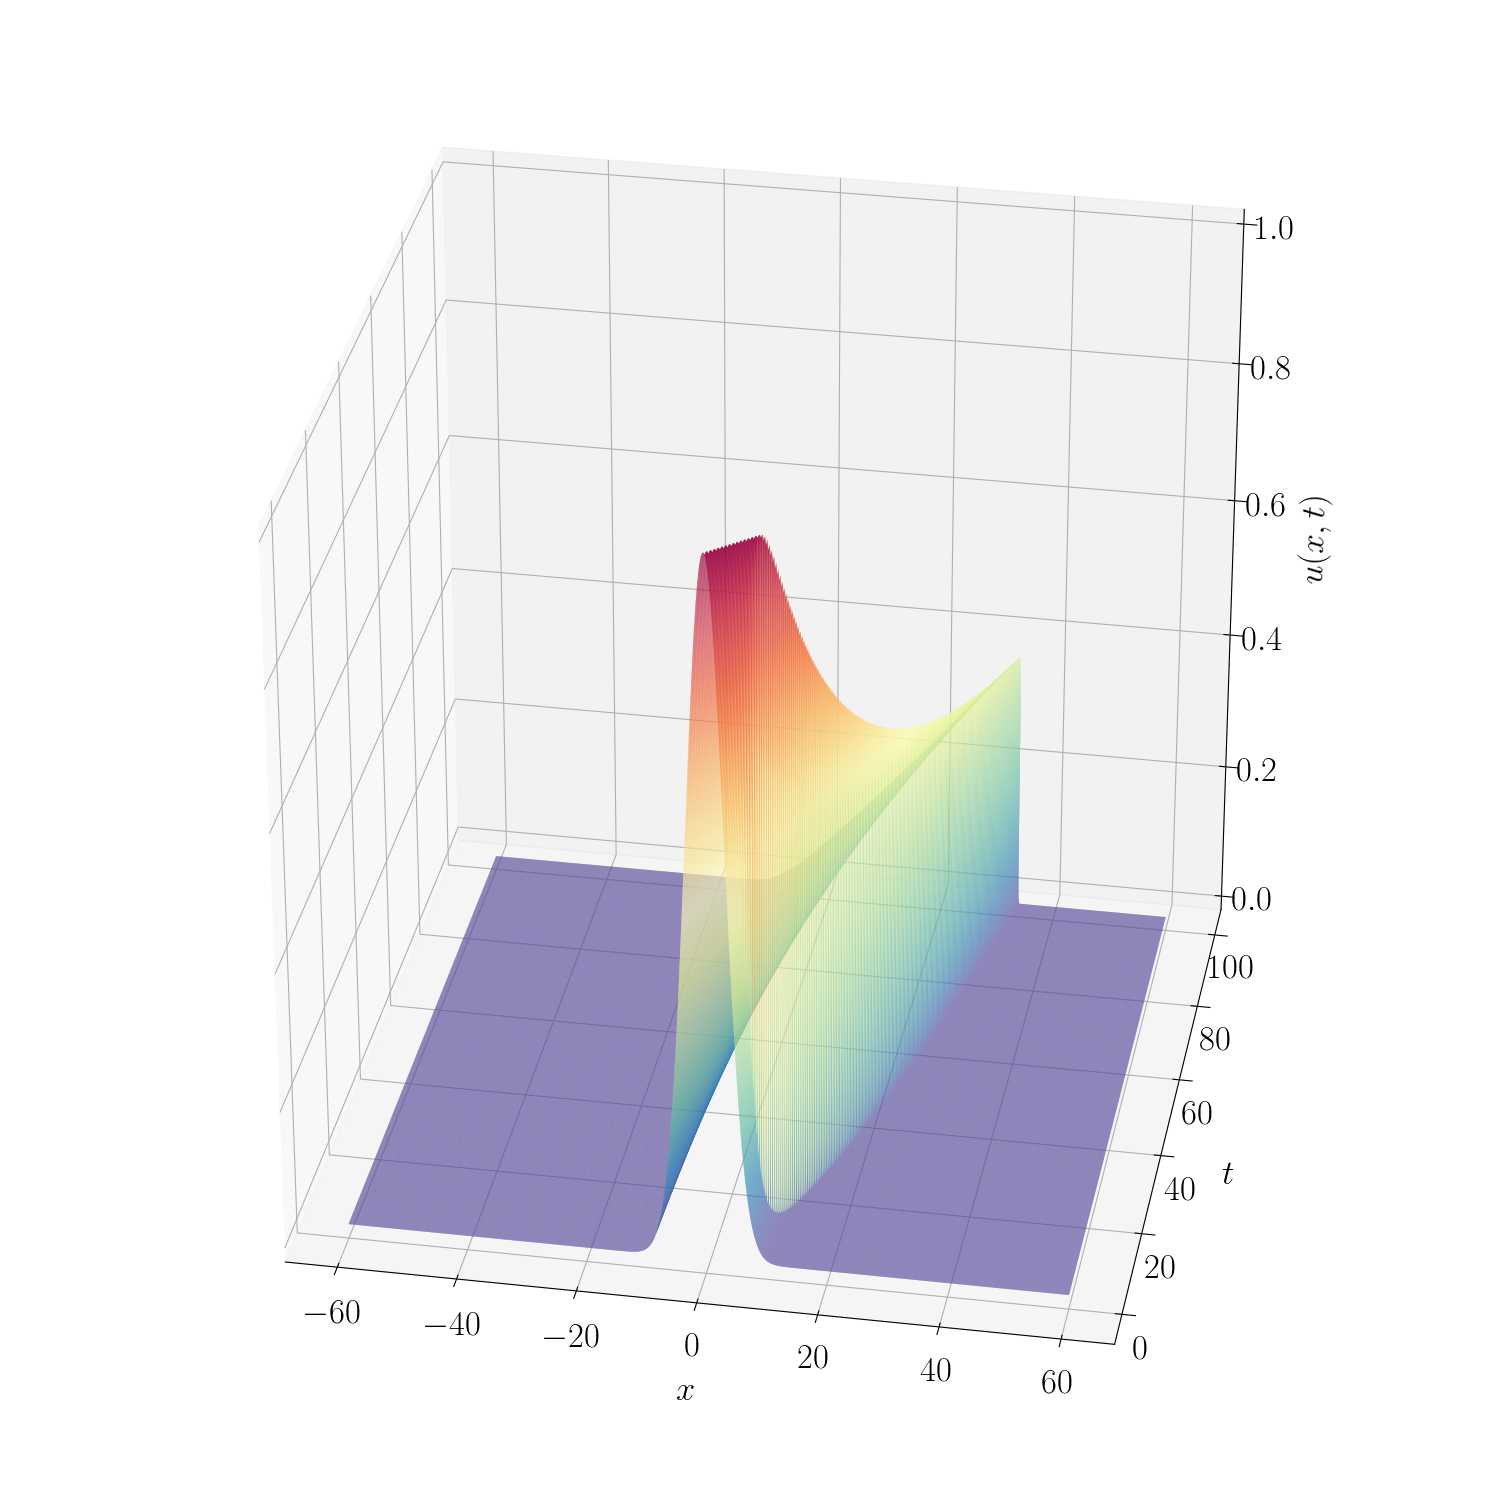
\includegraphics[width=7.5cm]{FIGURES/Galerkin/Graphics/eps=0.01/Exact_Solution_alpha=001.png}
\end{figure}
\end{frame}



\begin{frame}
	%Multiplying both sides of (\ref{strong}) by $\phi \in X$, for some appropriate space $X$ such that the integral of the PDE over the space $I$ is satisfied, we get   
	\only<1->{
	Simplificando notaci\'on:
	\begin{equation*}
	F(t, v) = \frac{1}{2} (v^2)_x - g(x, t), \hspace{3mm} A(v) = - \alpha v_{xx},
	\end{equation*}
		}
		\only<2->{
		\begin{equation*}
		\frac{\partial v}{\partial t} + A(v) + F(t, v) = 0, \hspace{2mm} t > 0.
	\end{equation*}
	}
	\only<3->{
	Con una adecuada elecci\'on de funciones de prueba $\phi \in X$	,
	\begin{block}{Formulaci\'on D\'ebil}	
	\begin{equation*}
	\displaystyle \int_{I} \frac{\partial v}{\partial t} \phi dx + \int_{I} A(v) \phi dx + \int_{I} F(t, v) \phi dx = 0, \hspace{2mm} \forall \phi \in X,\hspace{2mm} \forall t > 0.
	\end{equation*}
	\end{block}
	}
	\only<4->{
	\begin{block}{Formulaci\'on D\'ebil (Compacta)}	
	\begin{equation*}
	\left \langle \frac{\partial v}{\partial t} + A(v) + F(t, v), \phi\right\rangle = 0, \hspace{2mm} \forall \phi \in X, \hspace{2mm} \forall t > 0.
	\end{equation*}
	\end{block}
	}
\end{frame}
  
\section{M\'etodos Espectrales}
	\begin{frame}
\frametitle{M\'etodos Espectrales}
	\only<1->{
	Para la versi\'on determinista de este estudio nos enfocamos en el siguiente conjunto:
	\begin{equation*}
	\phi_n (x) = e^{inx}, \hspace{2mm} \displaystyle \int_{0}^{2\pi} \phi_k (x) \overline{\phi_l (x)} dx = 2 \pi \delta{kl}.
	\end{equation*}
	}
	\only<2->{
	\begin{block}{Coeficientes de Fourier} 
	\begin{equation*}
	\hat{u}_n = \frac{1}{2 \pi} \displaystyle \int_{0}^{2 \pi} u(x) e^{-inx} dx, \hspace{3mm}  k = 0, \pm 1, \pm 2, \dots, \hspace{2mm} u(x) \in L^2 [0, 2 \pi].
	\end{equation*}
	\end{block}	
	}
	\only<3->{
	\begin{block}{Series de Fourier}
		\begin{equation*}  
		F[u] \equiv \displaystyle \sum_{ |n| \leq \infty} \hat{u}_{n} e^{inx}.
		\end{equation*}
	\end{block}
	}
\end{frame}

\begin{frame}
	\only<1->{
	Definiendo	
	\begin{equation*}
		B = span\{e^{inx}: |n| \leq \infty \}
	\end{equation*}
	}
	\only<2->{
	\begin{block}{Operador de Proyecci\'on}	
	\begin{equation*}
	\mathcal{P}_N u(x) \equiv  \displaystyle \sum_{ |n| \leq \frac {N}{2}} \hat{u}_{n} e^{inx}.
	\end{equation*}
	\begin{equation*}
	\hat{B}_{N} = span \left\{e^{inx}: |n| \leq \frac {N}{2} \right\},\hspace{0.2cm} dim(\hat{B}_{N}) = N + 1.
	\end{equation*}	
	\end{block}	
	}
	\only<3->{
	Usando este operador nos facilita obtener derivadas
	\begin{equation*}
	\frac{d^q}{dx^q} \mathcal{P}_N u(x) = \displaystyle \sum_{ |n| \leq \frac {N}{2}} \hat{u}_{n} \frac{d^q}{dx^q} e^{inx} = \displaystyle \sum_{ |n| \leq \frac {N}{2}} (in)^q \hat{u}_{n}e^{inx}.
	\end{equation*}
	}
\end{frame}

\begin{frame}
	\only<1->{
	Otro operador utilizado en este estudio es definido por
	\begin{equation*}
	x_j = \frac{2 \pi j}{N + 1} , \hspace{0.5cm} j\in [0, \dots , N].
	\end{equation*}
	}
	\only<2->{
	Usando la regla de los trapecios
	\begin{equation*}
		\widetilde{u}_n = \frac{1}{N + 1}  \displaystyle \sum_{j = 0}^{N} u(x_j) e^{-in x_j},
	\end{equation*}
	}
	\only<3->{
	\begin{block}{Operador de Interpolacion}
		\begin{equation*}
			\mathcal{J}_N u(x) =  \displaystyle \sum_{ |n| \leq \frac {N}{2}} \widetilde{u}_n e^{inx}.
		\end{equation*}
	\end{block}
	}
\end{frame}

\begin{frame}
	\only<1->{
	La diferenciacion tambien es posible mediante
	\begin{equation*}
		\frac{d}{dx} \mathcal{J}_N u(x) = \displaystyle \sum_{|n| \leq N/2} in \widetilde{u}_n e^{inx}, \hspace{2mm} \widetilde{u}_n = \displaystyle \frac{1}{N + 1} \sum_{j=0}^{N} u(x_j) e^{-in x_j}.   
	\end{equation*} 
	}
	\only<2->{
	Otra manera m\'as pr\'actica es reescribiendo el operador:
	\begin{equation*}
		\mathcal{J}_N u(x) =  \displaystyle \sum_{j=0}^{N} u(x_j) h_j (x), \hspace{2mm} 	h_j (x) = \frac{1}{N + 1} \frac{\sin(\frac{N+1}{2}(x - x_j))}{\sin(\frac{x - x_j}{2})}
	\end{equation*}
	}
	\only<3->{
	\begin{block}{Matriz de Diferenciaci\'on}
	\begin{equation*}
		\label{matrix_DN_odd}
		\widetilde{D}_{ij} = \begin{cases} -\frac{(-1)^{i+j}}{2} \left[\sin \left[ \frac{x_i - x_j}{2}\right]\right]^{-2} &   i \neq j, \\ \hspace{15mm} 0 &  i=j. \end{cases}
	\end{equation*}
	\end{block}
	}
\end{frame}


\section{Ecuaci\'on de Burgers' Determinista}
\subsection{Galerkin}
\begin{frame}
	\only<1->{
	\begin{block}{Ecuacion de Burgers' Determinista}
		\begin{equation*}
		\frac{\partial u(x, t)}{\partial t} +  \frac{1}{2} \frac{\partial \left[ u(x, t) \right]^2}{\partial x} - \alpha \frac{\partial^2 u(x, t)}{\partial x^2} = 0.
		\end{equation*}
	\end{block}
	}
	\only<2->{
	Usando el operador proyecci\'on
	\begin{equation*}
	u_N (x, t) = \displaystyle \sum_{ |n| \leq \frac{N}{2} } \hat{u}_n e^{inx} 
	\end{equation*}
	}
	\only<3->{
	\begin{block}{Aproximacion por Fourier-Galerkin}
		\begin{equation*}
		\left \lbrace \begin{array}{ll}
		u_N(t): [0, T] \rightarrow V_N, \hspace{2mm} \text{t.q para cada} \hspace{2mm} \phi \in V_N \\
		\\
		( \frac{\partial u_N}{\partial t} + \frac{1}{2} (u_N^2)_x -  \alpha \frac{\partial^2 u_N}{\partial x^2}, \phi) = 0 \\
		\\
		u_N(0) = \mathcal{P}_N u_0 (x)
		\end{array}  \right .
		\end{equation*}
	\end{block}
	}
\end{frame}

\begin{frame}
	\only<1->{
	\begin{equation*}
	\displaystyle \frac{1}{2\pi} \int_{0}^{2 \pi} \left( \frac{\partial u_{N}}{\partial t} + \frac{1}{2} \frac{\partial}{\partial x} \left( u^2_N \right) - \alpha \frac{\partial^2 u_N}{\partial x^2} \right) e^{inx} dx = 0, \hspace{0.3cm} \forall |n| \leq \frac{N}{2} 
	\end{equation*}
	}
	\only<2->{
	\begin{equation*}
	\frac{d \hat{u}_n (t)}{dt} = \alpha p^2 n^2 \hat{u}_n (t) - p \widehat{G}_n (t) , \hspace{0.3cm} \forall |n| \leq \frac{N}{2} 
	\end{equation*}
	}
	\only<3->{
	Discretizando la variable temporal $t$ en el intervalo $[0, T]$ 
	\begin{equation*}
	t_j = j \Delta t, \hspace{2mm} j = 0, 1, \dots, T.
	\end{equation*} 
	}
	\only<4->{
	y para la variable espacial $x$ en el intervalo $[x_L, x_R]$, definiendo $x_n = p z_n + x_L$, $p = \frac{x_R - x_L}{2 \pi}$,  
	\begin{equation*}
	z_n = \frac{2 \pi n}{N}, \hspace{2mm} n = 0, 1, \dots, N.
	\end{equation*}
	}
\end{frame}

\begin{frame}
	\begin{block}{Discretizaci\'on Semi-Impl\'icita}
	\begin{equation*}
	\hat{u}_n (t_{j+1}) = \hat{u}_n (t_j) + \Delta t \left[\alpha p^2 n^2 \hat{u}_n (t_j) - p \widehat{G}_n (t_{j+1})  \right],
	\end{equation*}
	Donde $\widehat {G}_n $ 
	\begin{equation*}
	\widehat{G}_n (t_{j+1}) = \displaystyle in \left[ \sum_{|k| \leq \frac {N}{2}} \hat{u}_n (t_{j+1}) \hat{u}_{n - k} (t_{j+1}) \right].
	\end{equation*}
	\end{block}
\end{frame}

\begin{frame}
	\only<1->{	
	Finalmente es evaluada la solucion numerica
	\begin{equation*}
	u_N(x, t_j) = \displaystyle \sum_{|n| \leq \frac{N}{2}} \hat{u}_n (t_j) e^{inx}
	\end{equation*}
	}
	\only<2->{
	Para los siguientes resultados numericos se considero lo siguiente	
	\begin{equation*}
		u_0 (x) = e^{-0.05 x^2}, \hspace{3mm} x \in [-60, 60], \hspace{2mm} t \in [0, 100]. 
	\end{equation*}
	}
\end{frame}

\begin{frame}	
	\centering
	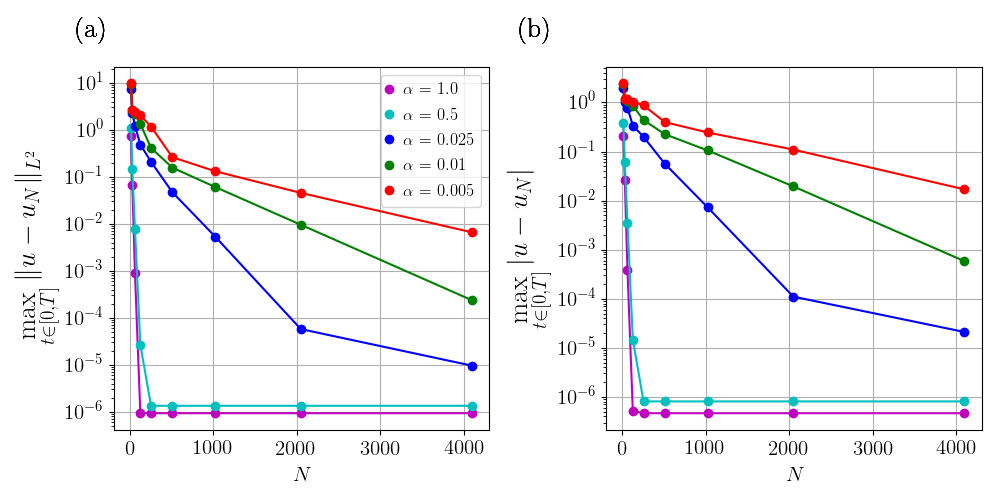
\includegraphics[width=11cm]{FIGURES/Galerkin/Graphics/alphas_Error_N.png}
	$N = 2^m$, $m = 4, \dots, 12$; $\Delta t = 1.0 \times 10^{-5}$.
\end{frame}
\begin{frame}	
	$\alpha = 1.0$; $N=2048$; $\Delta t = 1.0 \times 10^{-5}$.
	\centering
	\includegraphics[width=7.5cm]{FIGURES/Galerkin/Graphics/eps=1.0/Numerical_Solution_alpha=1.png}
\end{frame}
\begin{frame}
	$t = 100$, $\alpha = 1.0$, $\Delta t = 1.0 \times 10^{-5}$.
	\centering
	\includegraphics[width=10cm]{FIGURES/Galerkin/Graphics/eps=1.0/Numerical_Solution_alpha=1_T=100.png}
\end{frame}

\begin{frame}
\begin{table}
	\centering
	\begin{tabular}{lcccc}
		\toprule
		\multicolumn{1}{c}{\textbf{Approximation}} & \multicolumn{4}{c}{\textbf{Error}} \\
		$\hspace{9mm}N$ & $\Delta t=1\times 10^{-2}$ & $\Delta t=1\times 10^{-3}$ & $\Delta t=1\times 10^{-4}$ & $\Delta t=1\times 10^{-5}$ \\
		\midrule
		\hspace{7mm} 16 & 0.72504    & 0.72504    & 0.72504    & 0.72504    \\
		\midrule
		\hspace{7mm} 32 & 6.90249 $\times 10 ^{-2}$   & 6.88052 $\times 10 ^{-2}$   & 6.87838 $\times 10 ^{-2}$   & 6.87816 $\times 10 ^{-2}$   \\
		\midrule
		\hspace{7mm} 64 & 1.23827 $\times 10 ^{-3}$  & 8.85367 $\times 10 ^{-4}$ & 8.80521 $\times 10 ^{-4}$ & 8.80410 $\times 10 ^{-4}$  \\
		\midrule
		\hspace{7mm} 128 & 9.43454 $\times 10 ^{-4}$ & 9.41793 $\times 10 ^{-5}$ & 9.41148 $\times 10 ^{-6}$ & 9.41827 $\times 10 ^{-7}$  \\
		\midrule
		\hspace{7mm} 256 & 9.43454 $\times 10 ^{-4}$ & 9.41793 $\times 10 ^{-5}$ & 9.41109 $\times 10 ^{-6}$ & 9.36411 $\times 10 ^{-7}$ \\
		\midrule
		\hspace{7mm} 512 & 9.43454 $\times 10 ^{-4}$ & 9.41793 $\times 10 ^{-5}$ & 9.41109 $\times 10 ^{-6}$ & 9.36411 $\times 10 ^{-7}$ \\
		\midrule
		\hspace{7mm} 1024 & $\ast$ & 9.41793 $\times 10^{-5}$ & 9.41109 $\times 10^{-6}$ & 9.36411 $\times 10^{-7}$              \\
		\midrule
		\hspace{7mm} 2048 & $\ast$ & $\ast$ & 9.41109 $\times 10^{-6}$ & 9.36411 $\times 10^{-7}$   \\
		\\
		\bottomrule
	\end{tabular}
\end{table}
\end{frame}

\begin{frame}
	$\alpha = 0.005$; $N=2048$; $\Delta t = 1.0 \times 10^{-5}$.
	\centering
	\includegraphics[width=7.5cm]{FIGURES/Galerkin/Graphics/eps=0.005/Numerical_Solution_alpha=0005.png}
\end{frame}
\begin{frame}
	$t = 100$; $\alpha = 0.005$; $\Delta t = 1.0 \times 10^{-5}$.
	\centering
	\includegraphics[width=10cm]{FIGURES/Galerkin/Graphics/eps=0.005/Numerical_Solution_alpha=0005_T=100.png}
\end{frame}

\begin{frame}
\begin{table}
	\begin{tabular}{lcccc}
		\toprule
		\multicolumn{1}{c}{\textbf{Approximation}} & \multicolumn{4}{c}{\textbf{Error}} \\
		$\hspace{9mm}N$ & $\Delta t=1\times 10^{-2}$ & $\Delta t=1\times 10^{-3}$ & $\Delta t=1\times 10^{-4}$ & $\Delta t=1\times 10^{-5}$ \\
		\midrule
		\hspace{7mm} 16 & 9.95328   & 9.91901    & 9.91597    & 9.91567    \\
		\midrule
		\hspace{7mm} 32 & 2.72607   & 2.70558    & 2.70347    & 2.70326    \\
		\midrule
		\hspace{7mm} 64 & 2.50343   & 2.45988    & 2.45543    & 2.45497    \\
		\midrule
		\hspace{7mm} 128 & 2.16142   & 2.06992    & 2.05918    & 2.05795    \\
		\midrule
		\hspace{7mm} 256 & 1.3658    & 1.19385    & 1.17602    & 1.17412    \\
		\midrule
		\hspace{7mm} 512 & 0.339826  & 0.265843   & 0.262164   & 0.261805   \\
		\midrule
		\hspace{7mm} 1024 & 0.161405  & 0.133743   & 0.131882   & 0.131699   \\
		\midrule
		\hspace{7mm} 2048 & 6.50292 $\times 10^{-2}$ & 4.70602 $\times 10^{-2}$ & 4.57371 $\times 10^{-2}$  & 4.56090 $\times 10^{-2}$  \\
		\midrule
		\hspace{7mm} 4096 & * & 7.26917 $\times 10^{-3}$ & 6.64157 $\times 10^{-3}$ & 6.60753 $\times 10^{-3}$ \\
		\\
		\bottomrule
	\end{tabular}
\end{table}
\end{frame}

\subsection{Colocacion}
\begin{frame}
	\only<1->{
	\begin{block}{Aproximacion por Fourier-Colocaci\'on}	
	\begin{equation*}
		\left \lbrace \begin{array}{ll}
		u_N(t): [0, T] \rightarrow V_N, \hspace{2mm} \text{t.q para cada} \hspace{2mm} \phi \in V_N  \\
		\\
		\left\langle \frac{\partial u_N}{\partial t}, \phi \right\rangle_N - \left\langle \frac{\partial^2 u_N}{\partial x^2}, \phi \right\rangle_N + \frac{1}{2} \left\langle \mathcal{J}_N (u_N^2)_x, \phi \right\rangle_N = 0, \hspace{2mm} t > 0, \hspace{2mm} x \in I \\
		\\
		u_N(0) = \mathcal{J}_N u_0 (x), \hspace{2mm} t = 0, \hspace{2mm} x \in I
		\end{array}  \right .
	\end{equation*}	
	\end{block}
	}
	\only<2->{
	\begin{equation*}
		u_N (x, t) =  \displaystyle \sum_{|n| \leq \frac {N}{2}} \widetilde{u}_n (t) e^{inx}, \hspace{2mm} x_j = \frac{2 \pi j}{N + 1}, \hspace{2mm} j\in [0, \dots , N]. 
	\end{equation*}
	}
	\begin{equation*}
	R_{N} (x_j, t) = \frac{\partial u_N}{\partial t} (x_j, t) - \frac{\partial^2 u_N }{\partial x^2} (x_j, t) + \frac{1}{2} \mathcal{J}_N \left(u^2_N \right)_x (x_j, t) = 0
	\end{equation*}
\end{frame}

\begin{frame}	
	\only<1->{
	Necesitamos resolver las $N + 1$ ecuaciones diferenciales con condiciones iniciales $u_N (x_j, 0) = u_0(x_j)$, pero primeramente hacemos la siguiente notacion:
	\begin{equation*}
		u_N (t) = (u_N (x_0 , t), u_N (x_1 , t), \dots , u_N (x_{N} , t))^T,
	\end{equation*} 
	
	\begin{equation*}
	\frac{d u_N (t)}{dt} + \frac{1}{2} D_N u^2_N (t) - D_N^2 u_N (t) = 0,
	\end{equation*}
	}
	\only<2->{
	\begin{block}{Discretizacion Semi-Implicita}	
	\begin{equation*}
		u_N (t_{i + 1} ) = u_N (t_i) + \Delta t \left[p^2 D_N^2 u_N (t_i) - \frac{1}{2} p D_N u^2_N (t_{i+1}) \right].
	\end{equation*}
	\end{block}
	}
\end{frame}

\begin{frame}
	\only<1->{
	Discretizacion de $t$ en $[0, T]$
	\begin{equation*}
		t_i = i \Delta t, \hspace{2mm} i = 0, 1, \dots, T,
	\end{equation*} 
	}
	\only<2->{
	Discretizacion espacial $x$ en $[x_L, x_R]$, $x_j = p z_j + x_L$, $p = \frac{x_R - x_L}{2 \pi}$
	\begin{equation*}
		z_j = \frac{2 \pi j}{2N + 1}, \hspace{2mm} n = 0, 1, \dots, N.
	\end{equation*}
	}
	\only<3->{
	Finalmente, evaluamos la solucion numerica
	\begin{equation*}
		u_N(x, t_i) = \displaystyle \sum_{|n| \leq N} \hat{u}_n (t_i) e^{inx}
	\end{equation*}
	}
	\only<4->{
	Como anteriormente, se considero lo siguiente para los siguientes resultados numericos
	\begin{equation*}
		u_0 (x) = e^{-0.05 x^2}, \hspace{3mm} x \in [-60, 60], \hspace{2mm} t \in [0, 100]. 
	\end{equation*}
	}
\end{frame}

\begin{frame}
	$N = 2^m$, $m = 4, \dots, 11$; $\Delta t = 1.0 \times 10^{-5}$.
	\centering
	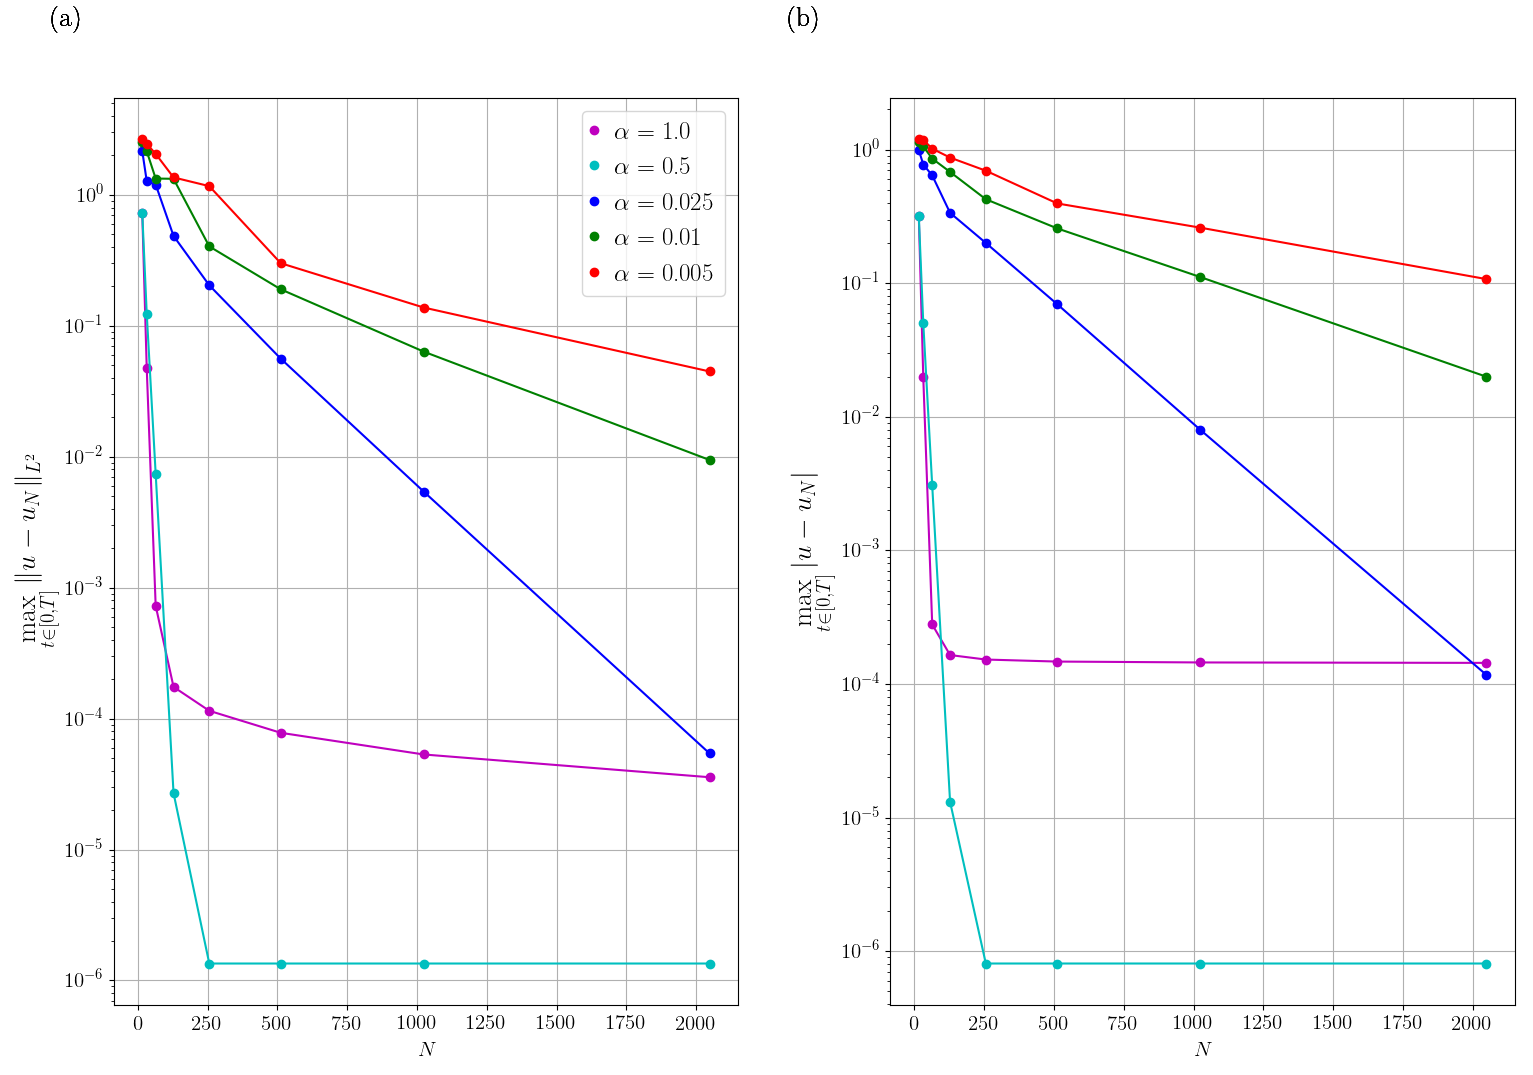
\includegraphics[width=9cm]{FIGURES/Collocation/collocation_alphas_N.png}
\end{frame}	

\begin{frame}
	$\alpha = 1.0$; $N=2048$; $\Delta t = 1.0 \times 10^{-5}$.
	\centering
	\includegraphics[width=7.5cm]{FIGURES/Collocation/Graphics/eps=1.0/Numerical_Solution_alpha=1.png}
\end{frame}
\begin{frame}
	$t = 100$, $\alpha = 1.0$, $\Delta t = 1.0 \times 10^{-5}$.
	\centering
	\includegraphics[width=10cm]{FIGURES/Collocation/Graphics/eps=1.0/Numerical_Solution_alpha=1_T=100.png}
\end{frame}

\begin{frame}
\begin{table}
	\begin{tabular}{lcccc}
		\toprule
		\multicolumn{1}{c}{\textbf{Approximation}} & \multicolumn{4}{c}{\textbf{Error}} \\
		$\hspace{9mm}N$ & $\Delta t=1\times 10^{-2}$ & $\Delta t=1\times 10^{-3}$ & $\Delta t=1\times 10^{-4}$ & $\Delta t=1\times 10^{-5}$ \\
		\midrule
		\hspace{7mm} 16 & 0.721112    & 0.721112    & 0.721112    & 0.721112    \\
		\midrule
		\hspace{7mm} 32 & 4.71797 $\times 10^{-2}$   & 4.72892 $\times 10^{-2}$   & 4.73004 $\times 10^{-2}$   & 4.73015 $\times 10^{-2}$   \\
		\midrule
		\hspace{7mm} 64 & 1.17954 $\times 10^{-3}$  & 7.35344 $\times 10^{-4}$ & 7.27561 $\times 10^{-4}$ & 7.27283 $\times 10^{-4}$  \\
		\midrule
		\hspace{7mm} 128 & 9.43454 $\times 10^{-4}$ & 1.75152 $\times 10^{-4}$ & 1.74583 $\times 10^{-4}$ & 1.74574 $\times 10^{-4}$ \\
		\midrule
		\hspace{7mm} 256 & 9.43454 $\times 10^{-4}$ & 1.15509 $\times 10^{-4}$ & 1.14669 $\times 10^{-4}$ & 1.14659 $\times 10^{-4}$ \\
		\midrule
		\hspace{7mm} 512 & 9.43454 $\times 10^{-4}$ & 9.41793 $\times 10^{-5}$ & 7.78847 $\times 10^{-5}$ & 7.78707 $\times 10^{-5}$ \\
		\midrule
		\hspace{7mm} 1024 & 0           & 9.41793 $\times 10^{-5}$ & 5.32213 $\times 10^{-5}$ & 5.32019 $\times 10^{-5}$ \\
		\midrule
		\hspace{7mm} 2048 & 0           & 0           & 3.56779 $\times 10^{-5}$ & 3.56498 $\times 10^{-5}$ \\
		\midrule
		\hspace{7mm} 4096 & 0           & 0           & 2.24122 $\times 10^{-5}$ & 0           \\
		\\
		\bottomrule
	\end{tabular}
\end{table}
\end{frame}

\begin{frame}
	$\alpha = 0.005$; $N=2048$; $\Delta t = 1.0 \times 10^{-5}$.
	\centering
	\includegraphics[width=7.5cm]{FIGURES/Collocation/Graphics/eps=0.005/Numerical_Solution_alpha=0005.png}
\end{frame}	
\begin{frame}
	$t = 100$, $\alpha = 1.0$, $\Delta t = 1.0 \times 10^{-5}$.
	\centering
	\includegraphics[width=10cm]{FIGURES/Collocation/Graphics/eps=0.005/Numerical_Solution_alpha=0005_T=100.png}
\end{frame}

\begin{frame}
\begin{table}
	\begin{tabular}{lcccc}
		\toprule
		\multicolumn{1}{c}{\textbf{Approximation}} & \multicolumn{4}{c}{\textbf{Error}} \\
		$\hspace{9mm}N$ & $\Delta t=1\times 10^{-2}$ & $\Delta t=1\times 10^{-3}$ & $\Delta t=1\times 10^{-4}$ & $\Delta t=1\times 10^{-5}$ \\
		\midrule
		\hspace{7mm} 16 & 1.36189   & 1.35883    & 1.35852   & 1.35849   \\
		\midrule
		\hspace{7mm} 32 & 2.67506   & 2.65305    & 2.65078   & 2.65055   \\
		\midrule
		\hspace{7mm} 64 & 2.50365   & 2.45855    & 2.45432   & 2.45387   \\
		\midrule
		\hspace{7mm} 128 & 2.15795   & 2.0632     & 2.05589   & 2.05497   \\
		\midrule
		\hspace{7mm} 256 & 1.362     & 1.18393    & 1.16697   & 1.16532   \\
		\midrule
		\hspace{7mm} 512 & 0.350775  & 0.304595   & 0.300865  & 0.300499  \\
		\midrule
		\hspace{7mm} 1024 & 0.168462  & 0.140332   & 0.13803   & 0.137804  \\
		\midrule
		\hspace{7mm} 2048 & 6.56161 $\times 10^{-2}$ & 4.63808 $\times 10^{-2}$  & 4.49226 $\times 10^{-2}$ & 4.47813 $\times 10^{-2}$ \\
		\midrule
		\hspace{7mm} 4096 & 0         & 7.66246 $\times 10^{-3}$ & 6.9909 $\times 10^{-3}$ & 0         \\
		\\
		\bottomrule
	\end{tabular}
\end{table}
\end{frame}

\subsection{Bajos Coeficientes de Viscosidad}
\begin{frame}
	\frametitle{Bajos Coeficientes de Viscosidad}
	\only<1->{
	Las siguientes soluciones, dadas por mediante Fourier-Galerkin, se considero
	\begin{equation*}
	u_0 (x) = e^{-0.005 x^2}, \hspace{3mm} x \in [-60, 60], \hspace{2mm} t \in [0, T_c], 
	\end{equation*}
	}
	\only<2->{
	donde
	\begin{equation*}
		Tc = \min_{x \in \mathbb{R}} \left[  \frac{-1}{u'_0 (x)} \right],
	\end{equation*}
	}
	\only<3->{
	tiempo donde ocurre una discontinuidad de la ecuacion
	\begin{equation*}
		\frac{\partial u(x, t)}{\partial t} +  \frac{1}{2} \frac{\partial \left[ u(x, t) \right]^2}{\partial x} = 0,
	\end{equation*}
	}
	\only<4->{
	la cual tiene como solucion
	\begin{equation*}
		u(x, t) = u_0 (x_0), \hspace{2mm} x_0 = x - u_0 (x_0) t, 
	\end{equation*}
	}
\end{frame}

\begin{frame}
	$t = T_c$; $N=256$; $\Delta t = 1.0 \times 10^{-3}$.
	\centering
	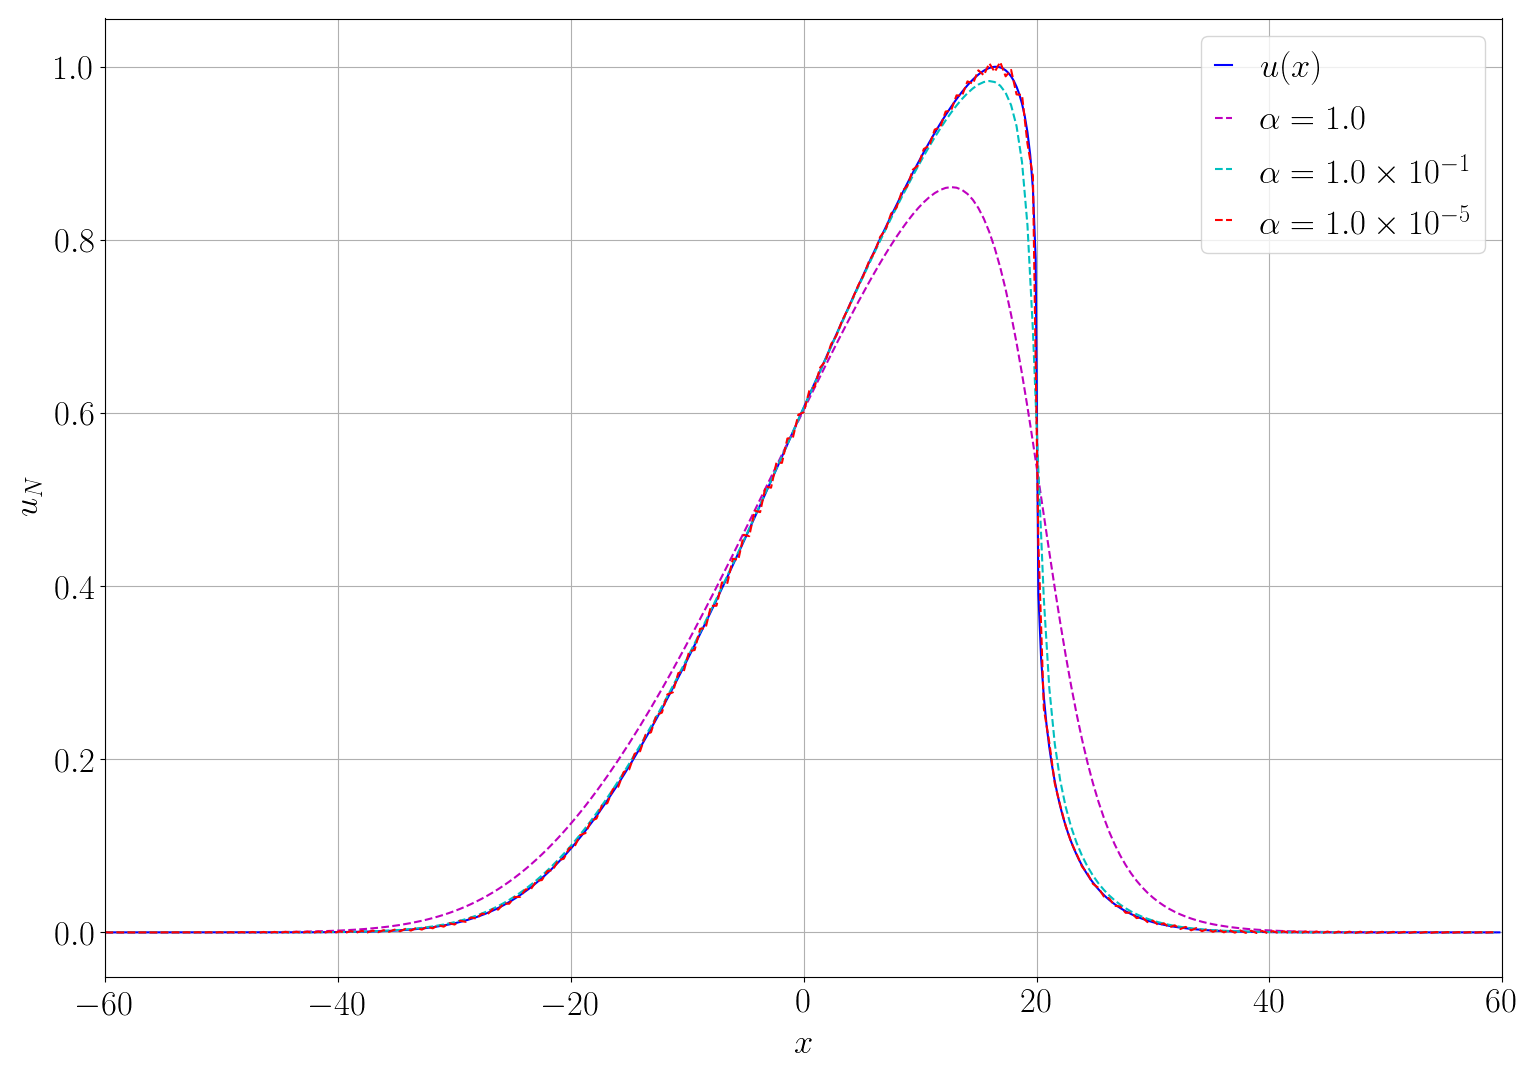
\includegraphics[width=10cm]{FIGURES/varios_alphas.png}
\end{frame}

\begin{frame}
	$\alpha = 1.0 \times 10^{-5}$; $N=256$;  $\Delta t = 1.0 \times 10^{-3}$.
	\centering
	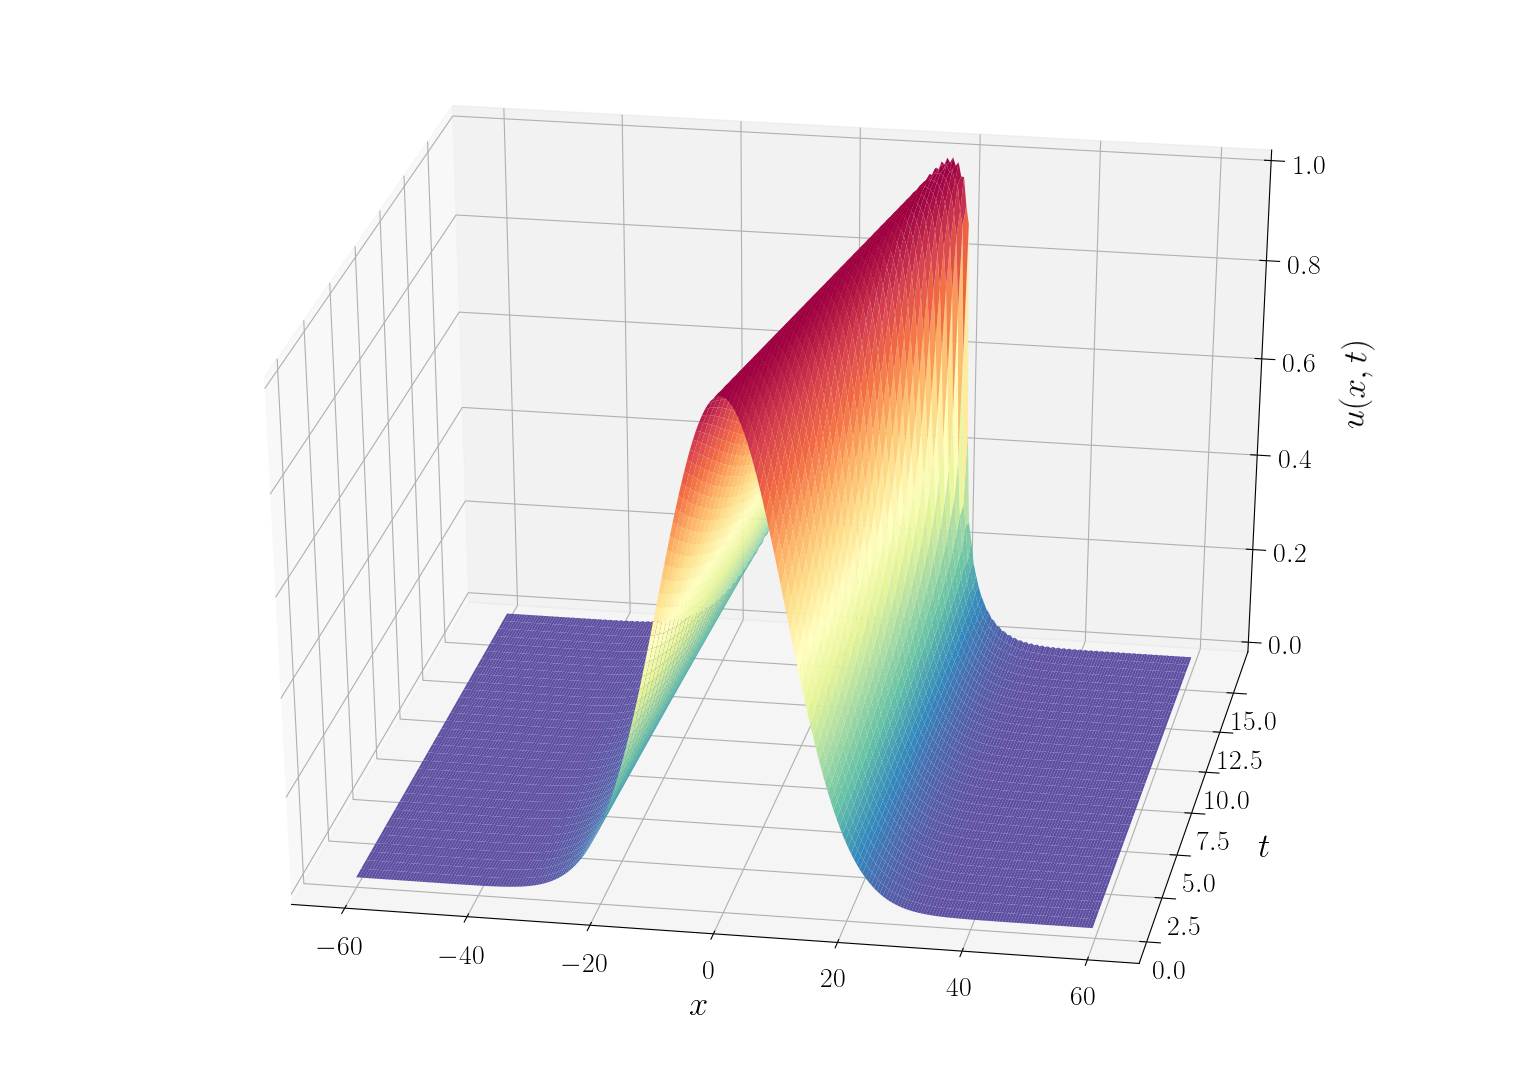
\includegraphics[width=10cm]{FIGURES/small_alpha.png}
\end{frame}

\begin{frame}
	 $t = T_c$; $\alpha = 1.0 \times 10^{-5}$; $\Delta t = 1.0 \times 10^{-3}$.
	\centering
	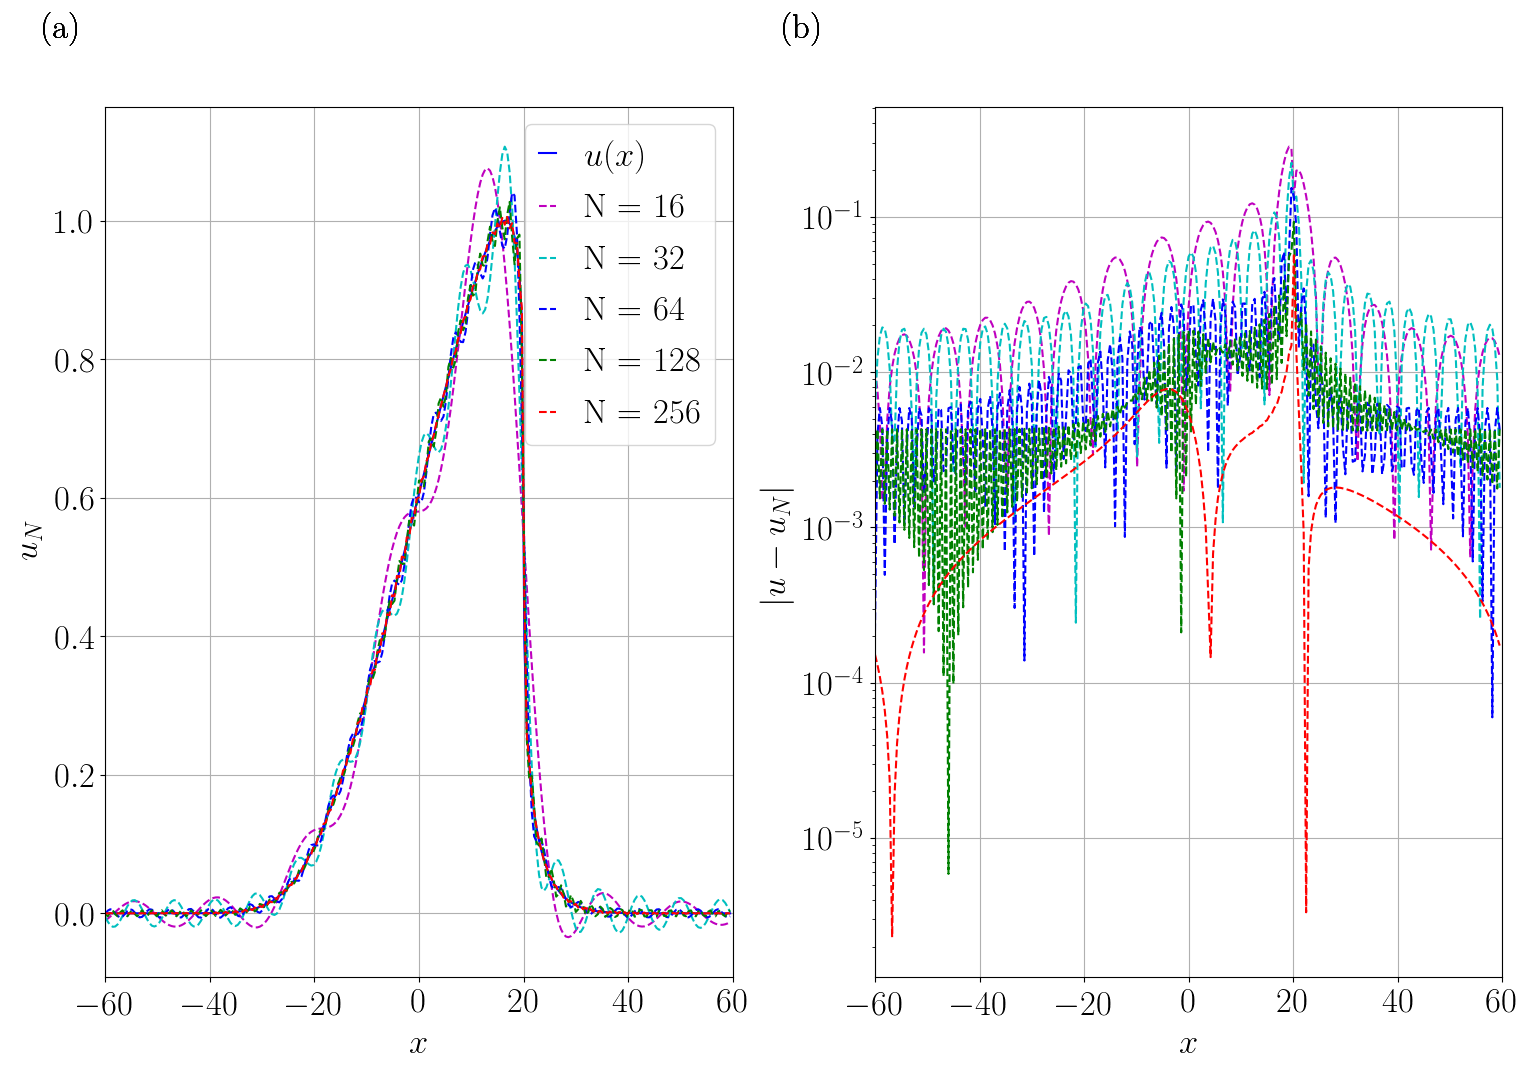
\includegraphics[width=10cm]{FIGURES/small_alpha_T.png}
\end{frame}

\begin{frame}
	\begin{table}
		\centering
		\begin{tabular}{lccc}
			\toprule
			\multicolumn{1}{c}{\textbf{Approximation}} & \multicolumn{3}{c}{\textbf{Distance}} \\
			\hspace{12mm} $N$ & $\Delta t=1\times 10^{-2}$ & $\Delta t=1\times 10^{-3}$ & $\Delta t=1\times 10^{-4}$ \\
			\midrule
			\hspace{12mm} 16 & 0.285531 & 0.285732 & 0.285752 \\
			\midrule
			\hspace{12mm} 32 & 0.222737 & 0.223260 & 0.223312 \\
			\midrule
			\hspace{12mm} 64 & 0.160385 & 0.162782 & 0.163025 \\
			\midrule
			\hspace{12mm} 128 & 0.129297 & 0.133322 & 0.133733 \\
			\midrule
			\hspace{12mm} 256 & 0.083291 & 0.091449 & 0.092320 \\
			\bottomrule
		\end{tabular}
	\end{table}
\end{frame}

\section{Ecuaci\'on de Burgers' Estoc\'astica}
  \begin{frame}
	\only<1->{
	\begin{block}{Ecuacion de Burgers' Estocastica}
	\begin{equation*}
		d X(\xi, t) = \left[\alpha \partial_{\xi}^2 X(\xi, t) + \frac{1}{2} \partial_\xi \left(X^2 (\xi, t)\right) \right] dt + dW_t (\xi, t), \hspace{0.2cm} \xi \in [0, 1] 
	\end{equation*}
	con las condiciones de frontera e iniciales
	\begin{align*}
		X(0, t) &= X(1, t) = 0 , \hspace{2mm} t > 0, \\
		X(\xi, 0) &= x(\xi), \hspace{2mm}  x \in \mathcal{H},
	\end{align*}
	\end{block}
	}
	\only<2->{
	La ecuacion anterior se asocia a la ecuacion estocastica
	\begin{align*}
		dX &= [AX + B(X)]dt + dW_t \\
		X(0) &= x, \hspace{0.2cm} x \in \mathcal{H}
	\end{align*}
	}
\end{frame}	

\begin{frame}	
	\only<1->{
	Primeramente para obtener la solucion numerica, se define la funcion
	\begin{equation*}
		u(x, t) = \mathbb{E} \left[ u_0 (X^x_t) \right], 
	\end{equation*}
	}
	\only<2->{
	 
	\begin{block}{Ecuacion de Kolmogorov}
	\begin{equation*}
		\frac{\partial u}{\partial t} = \frac{1}{2} Tr(QD^2 u) + \langle Ax, Du\rangle_{\mathcal{H}} + \langle B(x), Du\rangle_{\mathcal{H}}, \hspace{0.1cm} x \in D(A)
	\end{equation*}
	\end{block}
	}
\end{frame}

\begin{frame}
	La solucion espectral esta dada como
	\begin{align*}
		u(t, x) = \displaystyle \sum _{n \in \mathcal{J}} u_{n}(t) H_n (x), \hspace{0.1cm} x \in \mathcal{H}, \hspace{0.1cm} t \in [0, T],
	\end{align*}		
	
	substituyendo en la ecuacion de Kolmogorov 
	\begin{equation*}
		\dot{u}_{m} (t) = -u_{m} (t) \lambda_{m} + \displaystyle \sum _{n \in \mathcal{J}} u_{n} (t) C_{n, m} , \hspace{0.1cm} n, m \in \mathcal{J}
	\end{equation*}
	\begin{equation*}
		\mathcal{J} = \{\alpha = (\alpha_i,i \geq 1) | \alpha_i \in \mathbb{N}\cup \{0\}, |\alpha|:= \displaystyle \sum _{i = 0}^{\infty}\alpha_i < \infty\}
	\end{equation*}
\end{frame}

\begin{frame}	
	Para las soluciones numericas definimos 
	\begin{equation*}
		J^{M, N} = \{\gamma = (\gamma_i, \hspace{1mm} 1 \leq i \leq M  ) \hspace{1mm} | \hspace{1mm} \gamma_i \in \{0, 1, \cdots, N \} \}
	\end{equation*}
	
	Entonces la solucion truncada es 
	\begin{equation*}
		\hat{u}_N (x, t) = \displaystyle \sum_{ n \in J^{M, N} } u_n (t) H_n (x), \hspace{2mm} x \in \mathcal{H}, \hspace{2mm}, t \in [0, T].
	\end{equation*}
	
	para obtener
	\begin{equation*}
		\dot{u}_{m} (t) = -u_{m} (t) \lambda_{m} + \displaystyle \sum _{n \in S_N} u_{n} (t) \bar{C}_{n, m} , \hspace{0.1cm} n, m \in S_N
	\end{equation*}
\end{frame}
	
\begin{frame}	
	Reescribiendo el sistema
	\begin{equation*}
		U^M (t) =
		\begin{pmatrix}
		u_{m_1} (t) & u_{m_2} (t) & \dots & u_{m_M} (t)
		\end{pmatrix}^T   
	\end{equation*}
	\begin{equation*}
		\dot{U}^M (t) =
		\begin{pmatrix}
		\dot{u}_{m_1} (t) & \dot{u}_{m_2} (t) & \dots & \dot{u}_{m_M} (t)
		\end{pmatrix}^T   
	\end{equation*}
	
	\begin{equation*}
		A =
		\begin{pmatrix}
		-\lambda_1 + C_{1,1} & C_{2,1} & \dots & C_{M-1,1} & C_{M,1} 
		\\
		C_{1,2} & -\lambda_2 + C_{2,2} & \dots & C_{M-1,2} & C_{M,2}  
		\\
		\vdots & \vdots & \ddots & \vdots & \vdots
		\\
		C_{1,M-1} & C_{2,M-1} & \dots & -\lambda_{M-1} + C_{M-1,M-1} & C_{M,M-1} 
		\\
		C_{1,M} & C_{2,M} & \dots & C_{M-1,M} & -\lambda_{M} + C_{M,M} 
		\end{pmatrix}
	\end{equation*}
\end{frame}
	
\begin{frame}
	Representacion matricial del sistema
	\begin{equation*}
		\dot{U}^M (t) = AU^M (t)
	\end{equation*}
	La cual tiene como solucion
	\begin{equation*}
		U^M (t) = \displaystyle \sum _{j = 1}^{M} c_i V_i e^{\eta_i t}
	\end{equation*}
	
	Eigenvectores y eigenvalores
	\begin{align*}
		V &= a + i b \\
		\eta &= \beta + i \mu
	\end{align*}
\end{frame}

\begin{frame}
	\begin{equation*}	
	\begin{pmatrix}
	u_1 (0) \\ u_2 (0) \\ \vdots \\ u_{M-1} (0) \\	u_M (0)
	\end{pmatrix}
	= 
	\begin{pmatrix}
	V1 & V2 & \dots & V_{M-1} & V_M
	\end{pmatrix}
	\begin{pmatrix}
	c_1 \\ c_2 \\ \vdots \\ c_{M-1} \\ c_M
	\end{pmatrix}
	\end{equation*}
	
	\begin{equation*}
	\begin{pmatrix}
	c_1 \\ c_2 \\ \vdots \\ c_{M-1} \\ c_M 
	\end{pmatrix}
	=	
	\begin{pmatrix}
	V1 & V2 & \dots & V_{M-1} & V_M
	\end{pmatrix}^{-1}
	\begin{pmatrix}
	u_1 (0) \\ u_2 (0) \\ \vdots \\ u_{M-1} (0) \\	u_M (0)
	\end{pmatrix}
	\end{equation*}
\end{frame}

\begin{frame}
	En los siguientes resultados se considero $x(\xi)$ como condicion inicial, y su expansion truncada de Chebyshev como una segunda condicion inicial
	\begin{align*}
		x(\xi) = \sin(\pi \xi), \hspace{3mm} y(\xi) = \displaystyle \sum^{N}_{k=0} c_k T_k (\xi),
	\end{align*}
	Usando una discretizacion espacial $\xi$ de $2048$ puntos en el intervalo $[0, 1]$, $1024$ puntos en la variable $t$ sobre el intervalo $[0, 10]$, considerando los parametros $\alpha = 0.01$, $N = 5$, $M = 11$.
\end{frame}

\begin{frame}	
	\centering	
	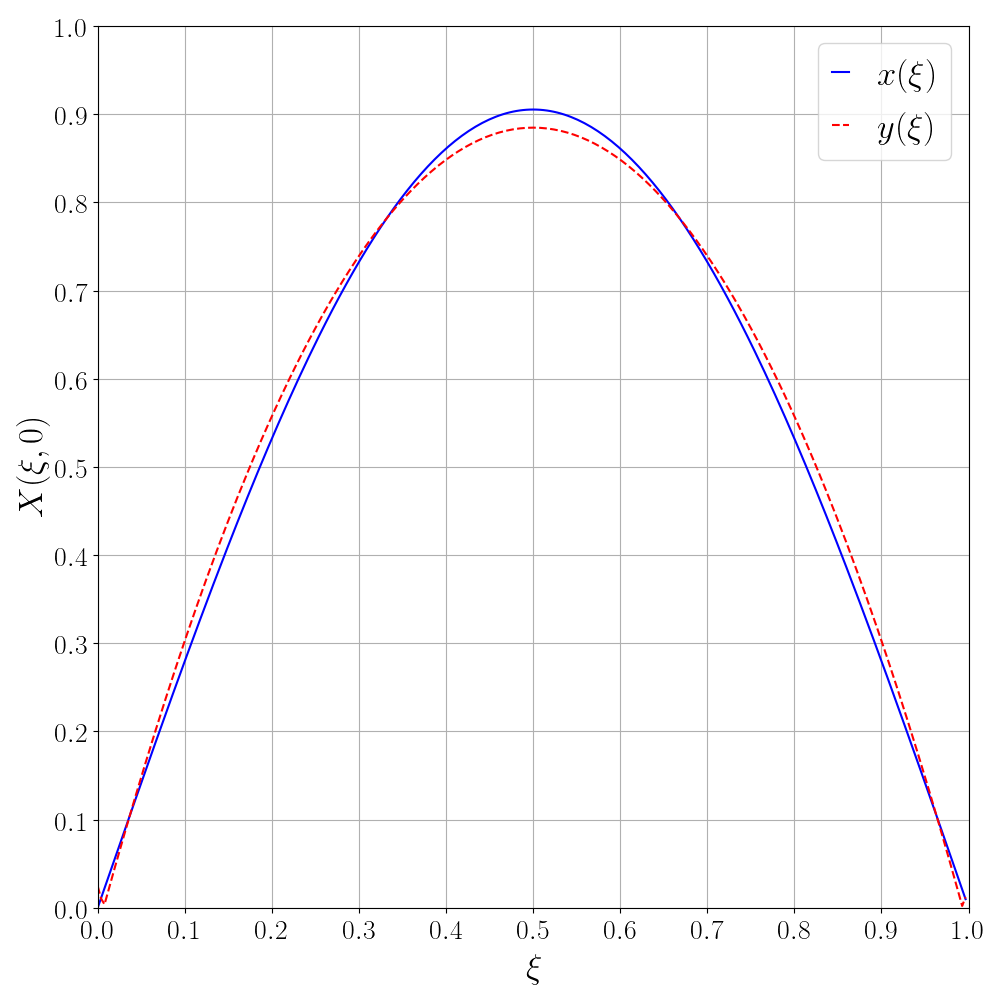
\includegraphics[width=8cm]{FIGURES/IC.png}
\end{frame}

\begin{frame}
	\centering
	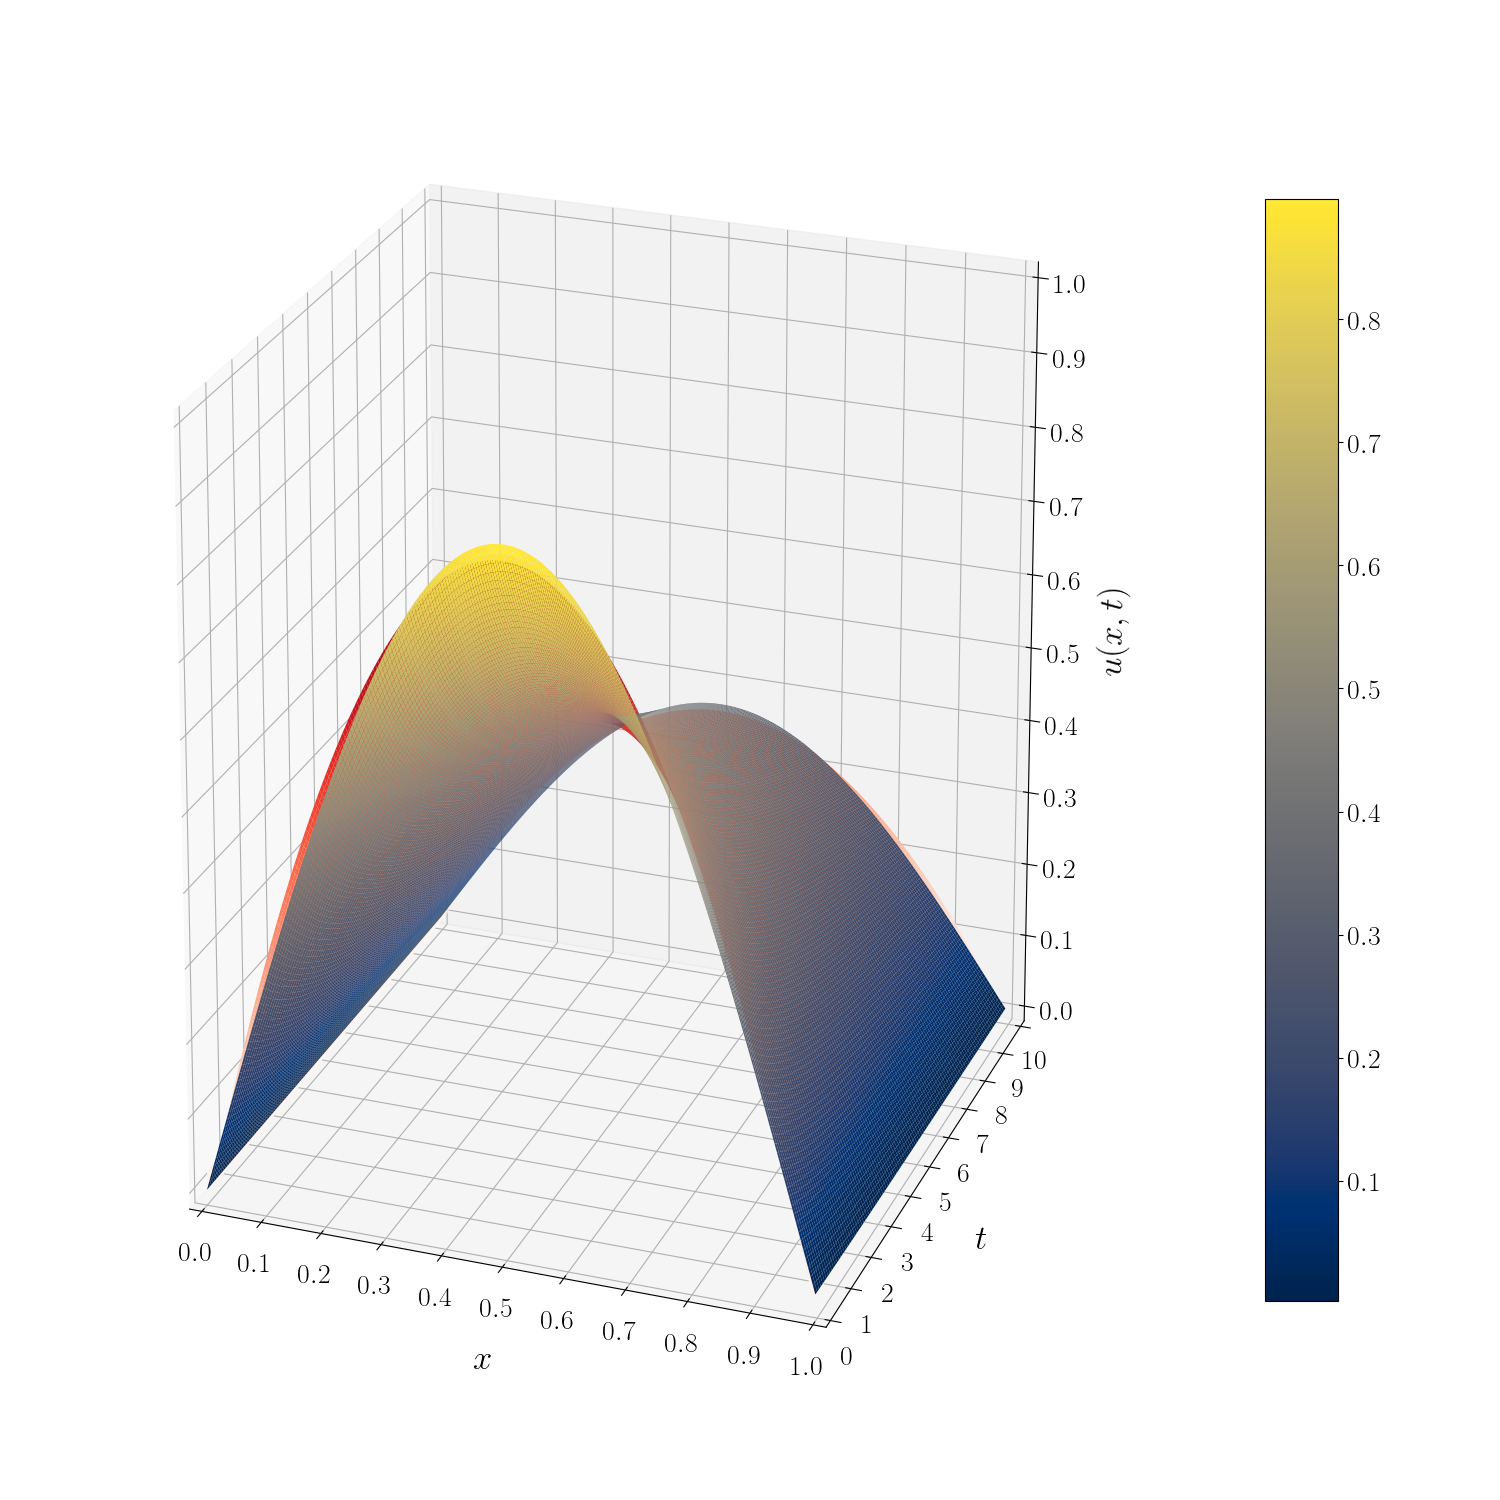
\includegraphics[width=8.5cm]{FIGURES/Numerical_Solution_Stochastic.png}
\end{frame}

\begin{frame}	
	\centering
	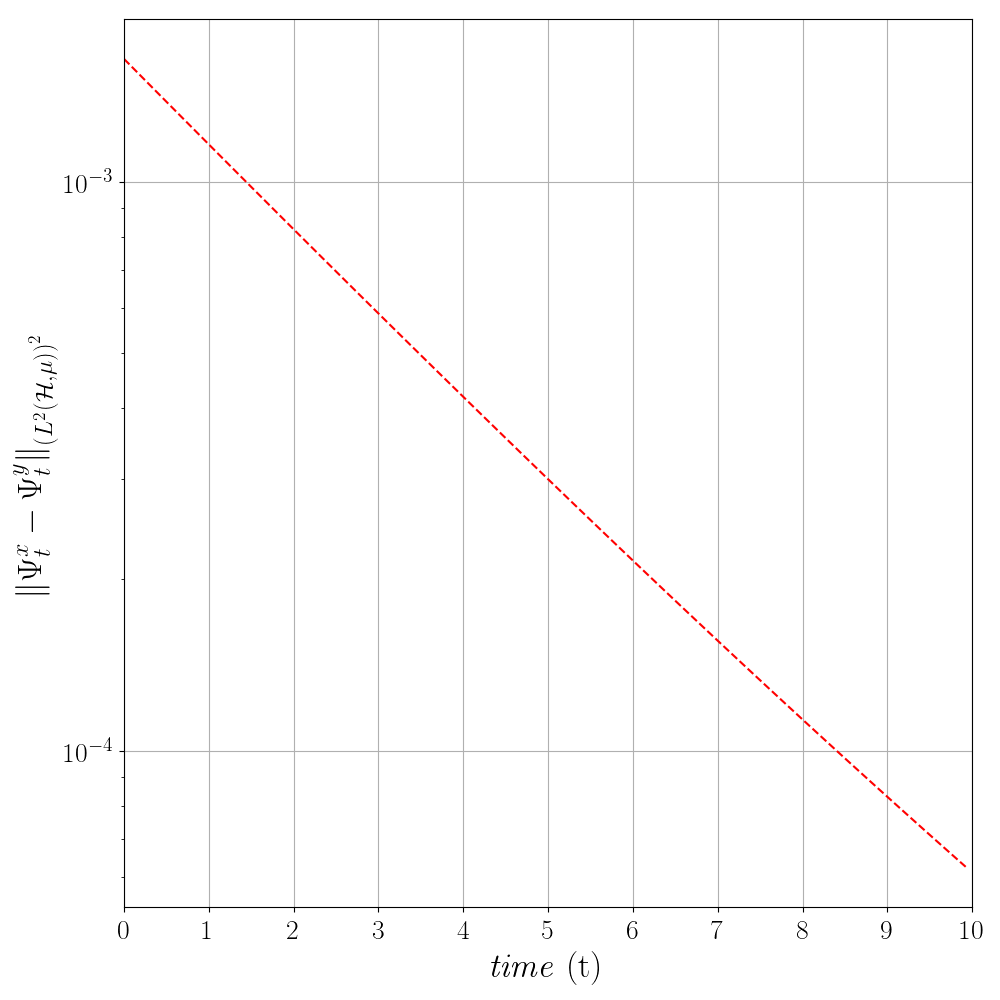
\includegraphics[width=7.5cm]{FIGURES/norms.png}
\end{frame}

\section{Conclusiones}
  \begin{frame}
\frametitle{Conclusiones}
	\begin{itemize}
		\only<1->{
		\item Los métodos espectrales son una excelente opción para resolver problemas donde las soluciones se comportan bien o son suficientemente suaves.
		}
		\only<2->{
		\item Pueden surgir desventajas en la práctica, como en los casos de coeficientes de viscosidad bajos, el orden de convergencia era menor.
		}
		\only<3->{
		\item Lo anterior se debió a una discontinuidad o cambios excesivos en la función.
		}
		\only<4->{
		\item De la misma manera con respecto a la versión estocástica de la ecuación de Burgers, y ademas son fáciles de implementar y desarrollar códigos computacionales muy eficientes. 
		}
	\end{itemize}
\end{frame}	

\end{document}
